\documentclass[11pt]{beamer}



\usepackage[utf8]{inputenc} %unix-windows-compatible
\usepackage{german}
\usepackage{fancyhdr} % Required for custom headers
\usepackage{lastpage} % Required to determine the last page for the footer
\usepackage{extramarks} % Required for headers and footers
%\usepackage[usenames,dvipsnames]{color} % Required for custom colors
\usepackage{graphicx} % Required to insert images
\usepackage{listings} % Required for insertion of code
\usepackage[section]{placeins}
\usepackage{caption} % to set figure captions in minipage
\usepackage{amsmath}
\usepackage{amssymb}
\usepackage{tikz}
\usetikzlibrary{matrix,chains,scopes,positioning,arrows,fit}
\usepackage{commath}
\usepackage{kpfonts}
\usepackage{algorithm}
\newcommand{\pushcode}[1][1]{\hskip\dimexpr#1\algorithmicindent\relax}
\usepackage[noend]{algpseudocode}

\usepackage{tcolorbox}
\usepackage{lipsum}

% (captionof{figure}{..}) Margins
%\topmargin=-0.45in
%\evensidemargin=0in
%\oddsidemargin=0in
%\textwidth=6.5in
%\textheight=9.0in
%\headsep=0.25in

%\linespread{1.1} % Line spacing
% tikz visibility on frames
\tikzset{
	invisible/.style={opacity=0},
	visible on/.style={alt={#1{}{invisible}}},
	alt/.code args={<#1>#2#3}{%
		\alt<#1>{\pgfkeysalso{#2}}{\pgfkeysalso{#3}} % \pgfkeysalso doesn't change the path
	},
}
% Set up the header and footer



\newtheorem{mydef}{Definition}
\newtheorem{theo}{Proposition}
\newtheorem{cor}{Corollary}


\makeatother
\setbeamertemplate{footline}
{
	\leavevmode%
	\hbox{%
		\begin{beamercolorbox}[wd=.4\paperwidth,ht=2.25ex,dp=1ex,center]{author in head/foot}%
			\usebeamerfont{author in head/foot}\insertshortauthor
		\end{beamercolorbox}%
		\begin{beamercolorbox}[wd=.6\paperwidth,ht=2.25ex,dp=1ex,center]{title in head/foot}%
			\usebeamerfont{title in head/foot}\insertshorttitle\hspace*{3em}
			\insertframenumber{} / \inserttotalframenumber\hspace*{1ex}
		\end{beamercolorbox}}%
		\vskip0pt%
	}
	\makeatletter
	\setbeamertemplate{navigation symbols}{}
	
	\AtBeginSection[]
	{
		\begin{frame}[plain]
			\frametitle{Table of Contents}
			\tableofcontents[currentsection]
		\end{frame}
	}
	
	
\begin{document}


	\title %optional
	{Enhanced Exact Algorithms for Discrete Bilevel Linear Problems	}
	\subtitle{Seminar: Selected Topics in Bilevel Optimization}
	
	\author % (optional, for multiple authors)
	{Leon Eifler}
	
	\institute % (optional)
	{
	
		Institut f"ur Mathematik\\
		Technische Universit"at Berlin
		
	}
	
	\date % (optional)
	{13.05.2016}
	

	\begin{frame}[plain]
	\titlepage

	\end{frame}
	
\AtBeginSection[]
{
	\begin{frame}[plain]
		\frametitle{Table of Contents}
		\tableofcontents[currentsection]
	\end{frame}
}

\begin{frame}
	\frametitle{Table of Contents}
	\tableofcontents
\end{frame}

\section{Introduction}

\begin{frame}	
	\frametitle{Problem}
	\begin{alignat*}{2}
		\text{(DBLP)} \quad \min_{x,y} F(x,y) &= c_1^Tx +c_2^Ty \\
		\text{s.t.} \quad &Cx + Dy \le e \\
		&x \in \mathbb{Z}^n_+ \\
		&y \in \arg \min_y f(y) &&= d^T y \\
		&\text{s.t.} &&Ax+By \le b \\
		& &&y \in \mathbb{Z}^m_+
	\end{alignat*}
\end{frame}

\begin{frame}
	\frametitle{Assumptions}
	\begin{itemize}
		\item No upper level constraints
		\item Optimistic approach
	\end{itemize}
\end{frame}

\begin{frame}
	\frametitle{Notation}
	\begin{itemize}
		\item \textit{Constrained Region}
		\begin{equation*}
		S = \{(x,y) | x \in \mathbb{Z}^m_+, y \in \mathbb{Z}^m_+, Cx+Dy \le e, Ax + By \le b \}
		\end{equation*}
		\item \textit{Followers Feasible Set}
		\begin{equation*}
			\Omega_y(x) = \{y| y \in \mathbb{Z}^m_+, By \le b - Ax \}.
		\end{equation*}
		\item \textit{Reaction Set}
		\begin{equation*}
			R_y(x) = \arg \min_y \{f(y) \ \text{s.t. } y \in \Omega_y(x).
		\end{equation*}
		\item \textit{Inducible Region}
		\begin{equation*}
			IR = \{(x,y)| x \in \mathbb{Z}^n_+, Cx+Dy \le e, y \in R_y(x)\}
		\end{equation*}
	\end{itemize}
\end{frame}

\begin{frame}
	\begin{columns}[T] % align columns
		\begin{column}{.48\textwidth}
			\tikzset{
	%Define standard arrow tip
	>=stealth',
	%Define style for different line styles
	help lines/.style={dashed, thick},
	axis/.style={<->},
	important line/.style={thick},
	connection/.style={thick, dotted},
}
\begin{tikzpicture}
	\coordinate (y) at (0,6);
	\coordinate (x) at (6,0);
	\draw[<->] (y) node[above] {$y$} -- (0,0) --  (x) node[right]{$x$};
	
	\foreach \x in {0,...,5}
	\draw (\x,1pt) -- (\x,-3pt)
	node[anchor=north] {\x};
	\foreach \y in {0,...,5}
	\draw (1pt,\y) -- (-3pt,\y) 
	node[anchor=east] {\y}; 

	\coordinate (A) at (1.278,3.444){};
	\coordinate (B) at (3.026,3.882){};
	\coordinate (C) at (3.986,3.210){};
	\coordinate (D) at (2.895,0.211){};
	
	\draw[important line] (A) node[left]{$A$} -- (B) node[above]{$B$}-- (C) node[right]{$C$} -- (D)node[right]{$D$} -- (A);
	
	\filldraw 
	(2,3) circle (1.5pt) node[align=right,   above] {a}
	(2,2) circle (1.5pt) node[align=right,   above] {b}
	(3,3) circle (1.5pt) node[align=right,   above] {c}
	(3,2) circle (1.5pt) node[align=right,   above] {d}
	(3,1) circle (1.5pt) node[align=right,   above] {e};
	
	\filldraw[fill=red, opacity=0.5, visible on=<2>] (A)  -- (B) -- (C)  -- (D) -- (A);
	\node[red, visible on = <2>] (S) at (2.5,5) {$S$};
	
	\filldraw[red, visible on=<3>] (2,2) circle(1.5pt);
	\filldraw[red, visible on=<3>] (2,3) circle(1.5pt);
	\filldraw[red, visible on=<3>] (2,1pt) -- (2,-3pt) node[anchor=north, red, visible on=<3>]{$2$};
	\node[red, visible on = <3>] (R) at (2.5,5) {$\Omega_y(2)$};
	
	\filldraw[red, visible on=<4>] (2,3) circle(1.5pt);
	\filldraw[red, visible on=<4>] (2,1pt) -- (2,-3pt) node[anchor=north, red, visible on=<4>]{$2$};
	\node[red, visible on = <4>] (R) at (2.5,5) {$R_y(2)$};
	
	\filldraw[red, visible on=<5>] (2,3) circle(1.5pt);
	\filldraw[red, visible on=<5>] (3,3) circle(1.5pt);
	\node[red, visible on = <5>] (R) at (2.5,5) {$IR$};
	\end{tikzpicture}
		\end{column}%
		\hfill%
		\begin{column}{.48\textwidth}
			\begin{alignat*}{2}
				\min_{x,y} F(&x,y) =&& 2x + 7y \\
				\text{s.t.}\quad &x \in \mathbb{Z}_+&& \\
				&y \in \arg&& \min_y f(y) = -y \\
				&\text{s.t.}\quad &&2x - 8y \ge -25 \\
				& &&7x + 10y \le 60 \\
				& &&2x + y \ge 6 \\
				& &&11x - 4y \le 31 \\
				& &&y \in \mathbb{Z}_+ 
			\end{alignat*}
		\end{column}%
	\end{columns}
	
\end{frame}

\begin{frame}
	\frametitle{Single Level Linear Problem}
	\begin{itemize}
	\item The Single Level Linear Problem is 
	\begin{align*}
		\text{(SLP)} \quad &\min_{x,y} F(x,y) = c_1^Tx +c_2^Ty \\
		&\text{s.t.} \quad (x,y) \in S.
	\end{align*}
	\item This is a relaxation of DBLP
	\item Dropping integrality and mantaining bilevel structure is not a relaxation
	\end{itemize}
\end{frame}

\section{A Cutting Plane Method}
\begin{frame}
	\frametitle{Cutting Plane Method}
	\begin{itemize}
		\item Solve (SLP). Get an integer solution $(\bar x, \bar y)$.
		\item If $(\bar x, \bar y)$ is bilevel infeasible, add valid inequality to eliminate bilevel-infeasible solutions at $\bar x$.
		\item Valid inequality is non linear but can be reformulated as bilevel and linear
		\item Cut turns (SLP) into bilevel problem with continuous follower variables. 
		\item This can again be transformed into a single-level problem
	\end{itemize}
\end{frame}

\begin{frame}
	\frametitle{Example Cutting Plane Method}
	\begin{columns}[T] % align columns
		\begin{column}{.48\textwidth}
			\tikzset{
	%Define standard arrow tip
	>=stealth',
	%Define style for different line styles
	help lines/.style={dashed, thick},
	axis/.style={<->},
	important line/.style={thick},
	connection/.style={thick, dotted},
}
\begin{tikzpicture}
	\coordinate (y) at (0,6);
	\coordinate (x) at (6,0);
	\draw[<->] (y) node[above] {$y$} -- (0,0) --  (x) node[right]{$x$};
	
	\foreach \x in {0,...,5}
	\draw (\x,1pt) -- (\x,-3pt)
	node[anchor=north] {\x};
	\foreach \y in {0,...,5}
	\draw (1pt,\y) -- (-3pt,\y) 
	node[anchor=east] {\y}; 

	\coordinate (A) at (1.278,3.444){};
	\coordinate (B) at (3.026,3.882){};
	\coordinate (C) at (3.986,3.210){};
	\coordinate (D) at (2.895,0.211){};
	
	\draw[important line] (A) node[left]{$A$} -- (B) node[above]{$B$}-- (C) node[right]{$C$} -- (D)node[right]{$D$} -- (A);
	
	\filldraw 
	(2,3) circle (1.5pt) node[align=right,   above] {a}
	(2,2) circle (1.5pt) node[align=right,   above] {b}
	(3,3) circle (1.5pt) node[align=right,   above] {c}
	(3,2) circle (1.5pt) node[align=right,   above] {d}
	(3,1) circle (1.5pt) node[align=right,   above] {e};
	
	\filldraw[red, visible on=<2>] (3,1) circle(1.5pt);
	\node[align=left, visible on=<2>] at (3,5){Optimal Solution of SLP \\ Not bilevel feasible};
	
	\draw[red, very thick, visible on=<3->] (3,0.5) -- (3,2.9);
	\node[align=left, visible on=<3>] at (3,5){Cut off all bilevel infeasible \\ solutions for this x};
	
	\filldraw[red, visible on=<4>] (2,2) circle(1.5pt);
	\node[align=left, visible on=<4>] at (3,5){Optimal Solution of new SLP};
	
	\filldraw[red, very thick, visible on=<5->] (2,2) -- (2,2.9);
	\node[align=left, visible on=<5>] at (3,5){Add new cut};
	
	\filldraw[red, visible on=<6>] (2,3) circle(1.5pt);
	\node[align=left, visible on=<6>] at (3,5){Optimal Solution of relaxation \\ is bilevel feasible};
	
	\end{tikzpicture}
		\end{column}%
		\hfill%
		\begin{column}{.48\textwidth}
			\begin{alignat*}{2}
			\min_{x,y} F(&x,y) =&& 2x + 7y \\
			\text{s.t.}\quad &x \in \mathbb{Z}_+&& \\
			&y \in \arg&& \min_y f(y) = -y \\
			&\text{s.t.}\quad &&2x - 8y \ge -25 \\
			& &&7x + 10y \le 60 \\
			& &&2x + y \ge 6 \\
			& &&11x - 4y \le 31 \\
			& &&y \in \mathbb{Z}_+ 
			\end{alignat*}
		\end{column}%
	\end{columns}
	\end{frame}
	
\begin{frame}
	\frametitle{The valid inequality}
	\begin{itemize}
		\item Assume solution of SLP is $(\bar x, \bar y)$ bilevel infeasible.
		\item There exists $(\bar x, \hat y)$ (bilevel feasible) with $f(\hat y) < f(\bar y)$.
		\item Valid inequality is 
		\begin{equation}
			f(y) \le f(\hat y) + L \|x-\bar x\|_{\infty}.
		\end{equation}
	\end{itemize}
\end{frame}
\begin{frame}
	\frametitle{Reformulation I}
	 The inequality ??? can be reformulated as 
		\begin{align*}
			f(y) \le f(\hat y) + L \hat z 
		\end{align*}
		where $\hat z$ is the optimal solution of 
		\begin{align*}
			(P_{\hat z}) \quad \min_{z} z \\
			\text{s.t.} \quad z &\ge x_i - \bar x_i \quad i = 1,\dots,n \\
			z &\ge \bar x_i - x_i \quad i = 1,\dots,n
		\end{align*}
\end{frame}

\begin{frame}
	\frametitle{Reformulation II}
	Adding this to SLP results in a bilevel continuous Problem 
\begin{alignat*}{2}
\text{(SLPC)} \quad &\min_{x,y} F(x,y)&& = c_1^Tx +c_2^Ty \\
&\text{s.t.} \quad (x,y)&& \in S. \\
&f(y) \le f(\hat y)&& + L \hat z \\
&\bar z \in \arg \min_{z}&& z \\
&  \text{s.t.} \quad &&z \ge x_i - \bar x_i \quad i = 1,\dots,n \\
& &&z \ge \bar x_i - x_i \quad i = 1,\dots,n \\
& && z \in \mathbb{R}
\end{alignat*}
This can again be reformulated as a single level problem.
\end{frame}

\section{A Branch and Cut Algorithm}
\begin{frame}
	\frametitle{Branch and Cut Method}
	\begin{itemize}
		\item Divide $S$ into smaller constrained regions $S', S''$.
		\item Solve both subproblems using Branch and Cut.
		\item Optimal solution is likely to be in $S'$. 
		\item $S''$ might be discarded based on relaxation and upper bound of $S'$.
	\end{itemize}
\end{frame}

\begin{frame}
	\frametitle{Motivation}
	\begin{theo}
		The inducible region of a bilevel linear problem can be written equivalently as a piecewise linear inequality constraint comprised of supporting hyperplanes of $S$.
	\end{theo}
	
	\tikzset{
	%Define standard arrow tip
	>=stealth',
	%Define style for different line styles
	help lines/.style={dashed, thick},
	axis/.style={<->},
	important line/.style={thick},
	connection/.style={thick, dotted},
}
\begin{tikzpicture}[scale=0.7]
	\coordinate (y) at (0,6);
	\coordinate (x) at (6,0);
	\draw[<->] (y) node[above] {$y$} -- (0,0) --  (x) node[right]{$x$};
	
	\foreach \x in {0,...,5}
	\draw (\x,1pt) -- (\x,-3pt)
	node[anchor=north] {\x};
	\foreach \y in {0,...,5}
	\draw (1pt,\y) -- (-3pt,\y) 
	node[anchor=east] {\y}; 

	\coordinate (A) at (1.278,3.444){};
	\coordinate (B) at (3.026,3.882){};
	\coordinate (C) at (3.986,3.210){};
	\coordinate (D) at (2.895,0.211){};
	
	\draw[important line] (A) node[left]{$A$} -- (B) node[above]{$B$}-- (C) node[right]{$C$} -- (D)node[right]{$D$} -- (A);
	
	\filldraw 
	(2,3) circle (1.5pt) node[align=right,   above] {}
	(2,2) circle (1.5pt) node[align=right,   above] {}
	(3,3) circle (1.5pt) node[align=right,   above] {}
	(3,2) circle (1.5pt) node[align=right,   above] {}
	(3,1) circle (1.5pt) node[align=right,   above] {};
	
	\draw[red, very thick, visible on = <1>] (A) -- (B) -- (C);
	\filldraw[red, visible on = <1>] (2,3) circle(1.5pt);
	\filldraw[red, visible on = <1>] (3,3) circle(1.5pt);
	
	\draw[blue, very thick, visible on=<2>] (0,3) -- (5,3);
	\draw[blue, very thick, visible on=<2>, visible on=<2>] (0,2) -- (5,2);
	\filldraw[fill=red, opacity = 0.5, visible on=<2>] (A) -- (B) -- (C) -- (3.909,3) -- (1.5,3) -- (A);
	\filldraw[fill=red, opacity = 0.5, visible on=<2>] (D) -- (2,2) -- (3.545,2) -- (D);
	
	\node[visible on = <2>] at (2.8,3.4){S'};
	\node[visible on = <2>] at (2.8,1.5){S''};	
	\end{tikzpicture}
\end{frame}

\begin{frame}
	\frametitle{Finding $S'$ and $S''$}
	\begin{itemize}
	\item We solve the max-min problem
		\begin{align*}
			(BLP^{max}_{min}) \quad \max_{x,y} f(y) &= d^T y \\
			\text{s.t.} \quad &x \in \mathbb{R}^n_{+} \\
			&y \in \arg \min_{y} f(y) = d^Ty \\
			&\text{s.t.} \quad Ax + By \le b \\
			& \quad y \in \mathbb{R}^m_{+}
		\end{align*}
		\item Let $(\hat x, \hat y)$ be optimal solution of $(BLP^{max}_{min})$
		\item Split $S$ into $S', S''$ by adding $f(y) \le \lceil f(\hat y) \rceil$ and $f(y) \ge \lceil f(\hat y) \rceil + 1$ respectively
	\end{itemize}
\end{frame}

\begin{frame}
	\frametitle{Branch and Cut for $S'$ and $S''$}
	We can solve the two subproblems using any branch and cut or cutting plane method method, i.e.:
	\begin{itemize}
		\item[Step 0]Determine $S'$ and $S''$.
		\item[Step 1]Solve the subproblem $(DBLP')$ induced by $S'$. Use continuous single-level relaxation. 
		\item[Step 2]Branch if solution is not integral, add cut if solution is integral but not bilevel feasible
		\item[Step 3]Compute $LB''$ for problem $(DBLP'')$ induced by $S''$. If this is worse than the $UB$ found before stop.
		Otherwise solve $(DBLP'')$.
	\end{itemize}
\end{frame}

\begin{frame}
	\frametitle{Proposed Variant}
	\begin{itemize}
		\item Use branch and cut to solve $(DBLP')$
		\begin{itemize}
			\item Use cuts that are computationally less expensive
			\item Intuition that $S'$ contains few bilevel-infeasible integral points
		\end{itemize}
		\item Use previosly introduced cutting plane method for $(DBLP'')$
		\begin{itemize}
			\item Yields strong bounds quickly
			\item Possibly prune whole subproblem
		\end{itemize}
	\end{itemize}
\end{frame}

\section{Computational Experiments}

\begin{frame}
	\frametitle{Setup}
	\begin{itemize}
		\item Compare with algorithm from DeNegre and Ralphs
		\item Testsets: Random instances and modified MIPLIB 2010 instances
		\item All algorithms implemented in C
		\item PC Pentium Core 2 Duo with a 2 GHz processor and 1 GB RAM
		\item Solver used is CPLEX 12.3
	\end{itemize}
\end{frame}
\begin{frame}
	\frametitle{Cutting Plane Algorithm}
	\begin{columns}[T]
		\begin{column}{.48\textwidth}
	\begin{figure}
		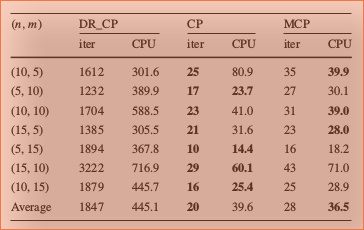
\includegraphics[width=\textwidth]{table_cp.png}
		\caption{Comparison on random set}
	\end{figure}
	\end{column}
	\begin{column}{.48\textwidth}
	\begin{figure}
		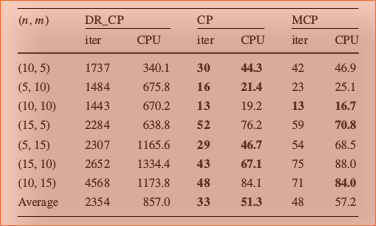
\includegraphics[width=\textwidth]{table_cp_miplip.png}
		\caption{Comparison on miplip set}
	\end{figure}
	\end{column}
	\end{columns}
\end{frame}

\begin{frame}
	\frametitle{Branch and Cut Algorithm}
	\begin{figure}
		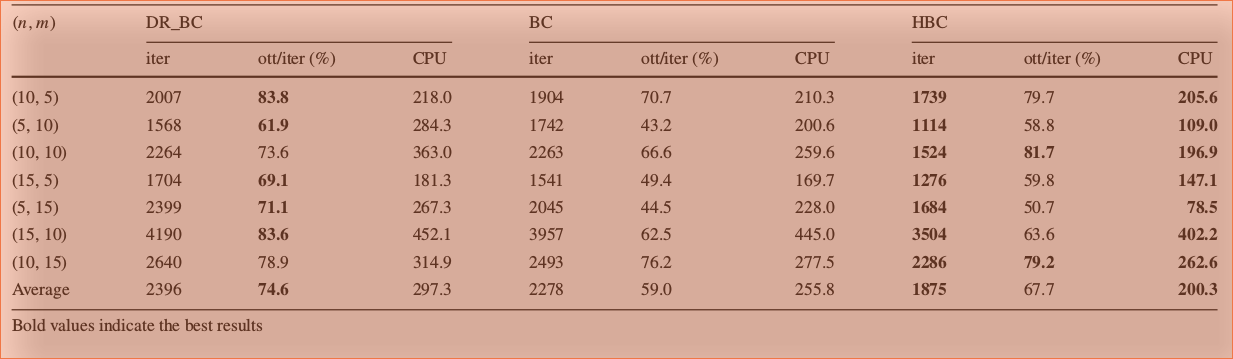
\includegraphics[width=\textwidth]{table_bc_random.png}
		\caption{Comparison on random set}
	\end{figure}
	\begin{figure}
		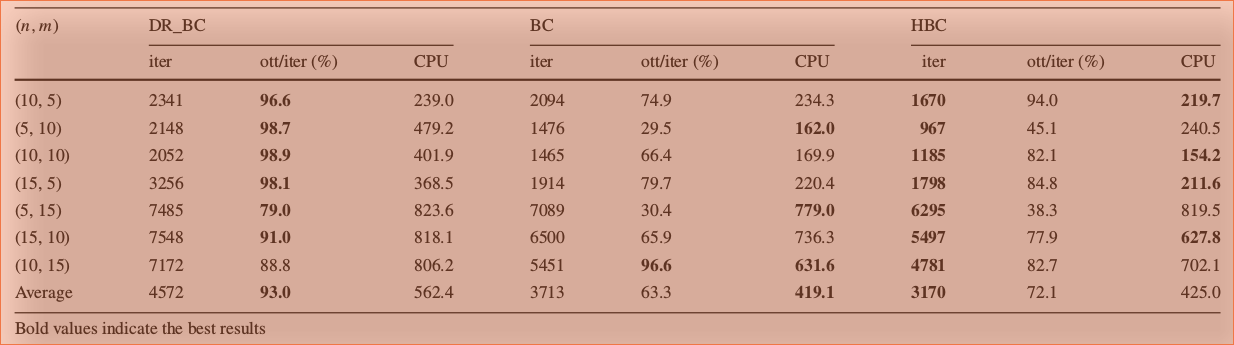
\includegraphics[width=\textwidth]{table_bc_miplip.png}
		\caption{Comparison on miplib set}
	\end{figure}
\end{frame}
\end{document}
